\documentclass[tikz]{standalone}

\usetikzlibrary{shapes}
\usetikzlibrary{angles}
\usetikzlibrary{calc} 

\usetikzlibrary{circuits.ee.IEC}

\usetikzlibrary{shadings}
\usetikzlibrary{fadings}
\usetikzlibrary{patterns}

\begin{document}

    
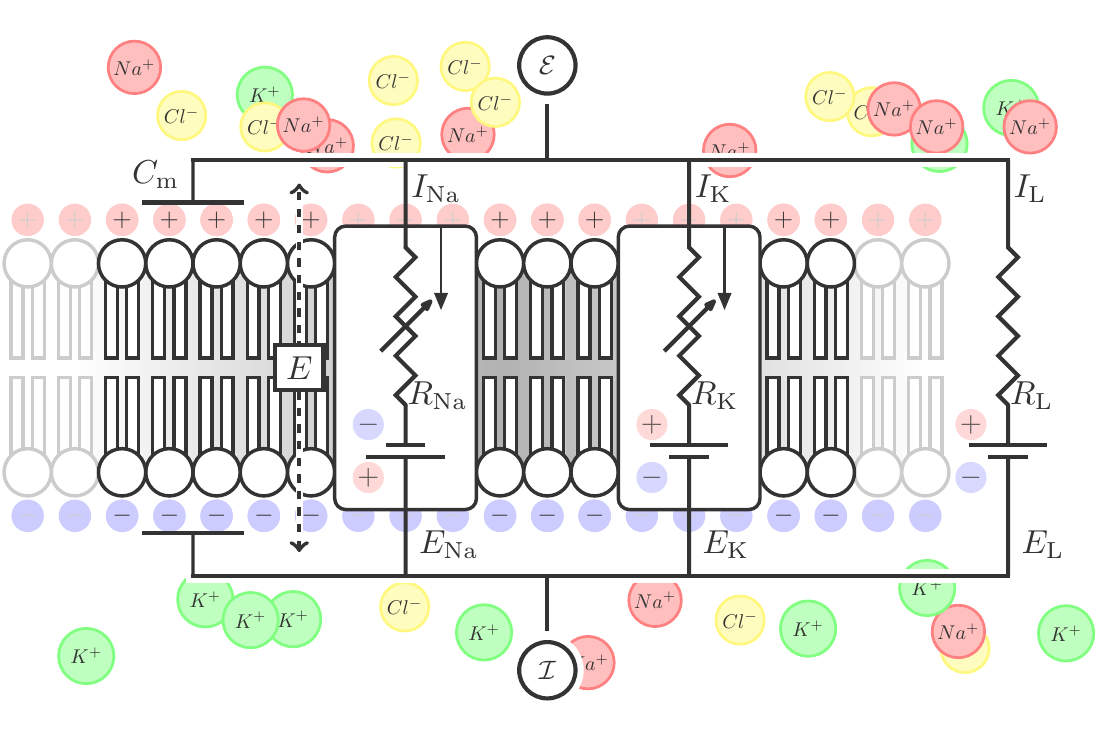
\begin{tikzpicture}[
    %x=1cm, y=1cm, 
    %z={(0cm,1cm)},
    scale = 1.2,
    transform shape,
    thick, 
    black!80,
    circuit ee IEC,
    every info/.style={font=\footnotesize},
        small circuit symbols,
            set resistor graphic=var resistor IEC graphic,
            set diode graphic=var diode IEC graphic,
            set make contact graphic= var make contact IEC graphic
    ]

    % Determines the boundries

    \tikzfading[name=fade outwards,
                left   color = transparent!100,
                right  color = transparent!100,
                middle color = transparent!0,
                ]
    \path[use as bounding box] (-5.5,-3.6) rectangle (5.5,3.6);
    \fill[color = black!30, path fading=fade outwards] (-5,-1.2) rectangle (4,1.2);
    
    
    \def\linWid{1 pt}
    
    \def\r{0.5}             % radius of heads
    \def\s{0.5}             % scale
    \def\l{2}               % length
    \def\w{0.75}            % width
    \def\wl{1}              % width of the lipids
    \def\wc{1.30}           % width of the capacitor
    \def\j{2cm}             % not too sure
    \def\chanGap{3cm}
    \def\exShift{3}
    \def\steps{4}

    % Ratio for each ion
    \def\Nar{3/10}
    \def\Kr{7/10}
    \def\Lr{11.5/10}
    \def\Nas{Na}
    %\def\Kr{3/12}
    %\def\Nar{7/12}
    %\def\Nar{1/(2*\r*\s)}
    \def\Clr{11/12}
    
    % Random number generation seed
    \def\seed{22061999}
    
    % Random Num shit
    \def\randomX#1{\pgfmathrandominteger{#1}{-600}{600}}
    \def\randomY#1{\pgfmathrandominteger{#1}{225}{330}}

    
    % Definining the coordinates of the box corners
    \def\boxRise{2.2}
    \def\boxRun{3.75}
    
    \coordinate (O)  at (0,0);
    \coordinate (TR) at ( \boxRun, \boxRise);
    \coordinate (TL) at (-\boxRun, \boxRise);
    \coordinate (BL) at (-\boxRun,-\boxRise);
    \coordinate (BR) at ( \boxRun,-\boxRise);

    % Define centers of the walls of the circuit
    \coordinate (CC) at ($(TL)!1/2!(BL)$);
    \coordinate (LC) at ($(TR)!1/2!(BR)$);
    
    % Define centers of the floor and ceiling of the circuit
    \coordinate (EM) at ($(TL)!1/2!(TR)$);
    \coordinate (IM) at ($(BL)!1/2!(BR)$);

    \fill[red] ;

        
    \def\phosLipid#1#2#3{
        \draw [fill = white, line width = 1.20pt, transform shape] (#1)+(-0.35*\wl,0) rectangle +(-0.1*\wl,-\l);
        \draw [fill = white, line width = 1.20pt, transform shape] (#1)+(+0.35*\wl,0) rectangle +(+0.1*\wl,-\l);
        \draw [fill = white, line width = 1.25pt, transform shape] (#1) circle (\r) 
                node[anchor = south, yshift = 15.5, inner sep = 1pt, circle, fill = #2!20!white, scale = 1.5] {$#3$};
    }

    \def\lipidBlock#1#2{
    \begin{scope}[xshift = #2]
        \begin{scope}[yshift = \exShift pt +\j*\s, scale = \s ]
            \foreach \i in {0,...,#1}{
                \phosLipid{ \i , 0 }{red}{+}
            }
        \end{scope}
        \begin{scope}[yshift = -\exShift pt -\j*\s, scale = \s, rotate = 180]
            \foreach \i in {0,...,-#1}{
                \phosLipid{ \i , 0  }{blue}{-}
            }
        \end{scope}
    \end{scope}
    }

    % Maps out certain coordinates in relation to the centers of the channels
    \path ($(CC)!\Nar!(LC)$) node {}; \pgfgetlastxy{\Nax}{\Nay}
    \path ($(CC)!\Kr!(LC)$)  node {}; \pgfgetlastxy{\Kx}{\Ky}
    %\path (Na+) -- +(0:\w * 2 cm + 2 * 2 * \r*\s cm) node (Cl-) {};\pgfgetlastxy{\Clx}{\Cly}

                
    \begin{scope}
    % random scattering of ions in background
    \pgfmathsetseed{\seed}
    \foreach \CYC/\SIGN in {3/-1,8/+1}{
        \foreach \i in {1,...,\CYC}{
            \foreach \NN/\CC/\WW/\SS in 
                {K^+/green/227/-, 
                 Na^+/red/166/+, 
                 Cl^-/yellow/79/+}{
                    \pgfmathrandominteger{\rX}{-550}{550}
                    \pgfmathrandominteger{\rY}{228}{325}
                    
                    \draw (\rX/100,\SIGN * \SS\rY/100)  
                    node[circle, fill = \CC!25!white, draw = \CC!50, line width = 1pt, inner sep = 2*\WW/227, scale = 0.6] {$\phantom{Na^+}$}
                    node[scale = 0.6] {$ {\NN} $}; 
                }
        }}
    \end{scope}
    
    % The ghostly lipids in the backgroun
    \begin{scope}[black!20, line width = 0.75pt, 
                  ]
    \foreach \N/\I in {  8/  \r*\s,
                          % 2/-\Nax/+ ,
                       -11/ -\r*\s }{
        \lipidBlock{\N}{0 cm}
    }
    \end{scope} 
    % The foreground lipids
    \foreach \N/\I/\S in { 1/ \Kx /+,
                           0/ \Kx /-,
                           1/ \Nax/+,
                          -4/ \Nax/- }{
        \lipidBlock{\N}{\I /1.2 \S \w  cm \S \r*\s cm }
    }

    % Creates the channels
    \foreach \i/\RGB in {\Kx/green,\Nax/red
                        %,\Clx/yellow
                        }{
           \node at (\i/1.2,0) [rectangle,
                            line width = 1.25,
                            rounded corners,
                            minimum height= 1.5 *\l cm,
                            minimum width = 2 *\w cm,
                            draw = black!80, 
                            fill = white,
                            ] {};
    }

    
    % Underlines Circuit
    \begin{scope}[white, line width = 5pt]
              
    % Leakage
    \draw ($(TL)!\Lr!(TR)$) to [resistor={pos = 0.40}, 
        battery={pos = 0.70, minimum height=0.75cm, minimum width=0.15cm, line cap = rect}]  %node [pos = 0.5, anchor = north west, xshift = -3.5]{$R_\mathrm{L}$} 
            ($(BL)!\Lr!(BR)$);

          
    % Outlines circuit
    \draw[line cap = rect] (TL) -- ($(TL)!\Lr!(TR)$) 
                           (BL) -- ($(BL)!\Lr!(BR)$);
    \end{scope}
        
    \begin{scope}[line width = 1.5pt] % Draws the visible circuit
        % Marks the extternal Nodes
        \path ( 90: \boxRise + 1)  node (E) [circle, minimum width = 0.77cm, fill = white]{};
        \path (-90: \boxRise + 1) node  (I) [circle, minimum width = 0.77cm, fill = white]{};

    
        % Node to Cicuit
        \draw[white, line width = 5pt] 
              (E) to (EM)
              (I) to (IM);

              
        % Node to Cicuit
        \draw (E) to (EM)
              (I) to (IM);

         % Node to Cicuit  
        \node at (I) [circle,draw, fill = white] {\footnotesize $\mathcal{I}$};
        \node at (E) [circle,draw, fill = white] {\footnotesize $\mathcal{E}$};
        
        % Outlines circuit
        \draw[line cap = rect] (TL) -- ($(TL)!\Lr!(TR)$) 
                               (BL) -- ($(BL)!\Lr!(BR)$);



        % Internal labeling and circutry
        \begin{scope}[align=left]
        \foreach \F/\I/\R/\A in 
            {\Nar/Na/0/adjustable', \Kr/K/180/adjustable', \Lr/L/180/}{
            % Making the main circuit paths
            \draw ($(BL)!\F!(BR)$) to 
            [battery={pos = 0.30, minimum height=1cm, minimum width=0.15cm, rotate = \R, line width = 1.2pt}, 
             resistor={\A, pos = 0.60, minimum height=0.25cm, minimum width = 2cm}] 
                node[pos = 0.5, anchor = north west, xshift = -3.5]
                {$R_\mathrm{\I}$} ($(TL)!\F!(TR)$);
    
            % Making external markings
            \path ($(TL)!\F!(TR)$) -- ($(BL)!\F!(BR)$) node (I\I) 
                [pos = 0.069, anchor = west, inner sep = 1pt]  
                {$I_{\mathrm{\I}}$};
            
            \path ($(TL)!\F!(TR)$) -- ($(BL)!\F!(BR)$) node (E\I) 
                [pos = 0.925, anchor = west]  
                {$E_{\mathrm{\I}}$};
    
            \foreach \o in {-,+}{
                \path ($(TL)!\F!(TR)$) -- ($(BL)!\F!(BR)$) 
                    node (S\I\o) [pos = 0.70, anchor = east, inner sep=0pt, xshift = -0.35cm, yshift = \o 0.28 cm]  {};
            }
        }
    
        % Arrows
        \foreach \i in {\Kr, \Nar}{
            \draw[line width = 1pt] ($(TL)!\i+0.05!(TR)$)++(0,-0.70cm) -- ++(0,-0.75cm) 
            node[isosceles triangle, scale = 0.25, draw, fill, rotate = 270] 
            {};
        }

        % Arrowing each side
        \path ($(BL)!\Nar/2!(BR)$) -- +(0, 0.25) coordinate (BE)
              ($(TL)!\Nar/2!(TR)$) -- +(0,-0.25) coordinate (TE);
        \end{scope}
        
        % Capacitance shit
        \draw[line cap = rect, line width = 1.2pt]  (BL) to 
            [capacitor={minimum height= \wc cm, minimum width = \l * \r * \s * 4 *1.2 cm + \exShift * \s * 1.2   cm}] (TL);
        \path (BL) -- (TL) node[near end, anchor = south east, yshift = 0.65cm] {$C_\mathrm{m}$};

        \path (CC)++( 90:\l * \s +  \r * \s  + \exShift * \s  cm) -- +(0:0.5*\wc) coordinate (PR) -- +(180:0.5*\wc) coordinate (PL);
        \path (CC)++(-90:\l * \s +  \r * \s  + \exShift * \s  cm) -- +(0:0.5*\wc) coordinate (NR) -- +(180:0.5*\wc) coordinate (NL);

    \end{scope}


    % Coloring the charges
    \begin{scope}[circle, inner sep=0.25pt, opacity = 0.75]
        \foreach \P in {0,0.25,0.50,0.75,1} \foreach \CR/\CL/\S/\RGB in {PR/PL/+/red, NR/NL/-/blue} {
            \path 
                (\CR) -- (\CL) node[pos = \P, fill = \RGB!20!white, opacity = 0.0] 
                {\footnotesize $\S$} 
                ;
        }
        \foreach \i in {Na, K, L}{
            \ifx\i\Nas
                \foreach \o/\s/\RGB in {-/+/red, +/-/blue}{
                     \path (S\i\o) node[fill = \RGB!20!white] 
                     {\footnotesize$\mathbf{\s}$} 
                     ;
            }
            \else
                \foreach \o/\RGB in {-/blue,+/red}{
                     \path (S\i\o) node[fill = \RGB!20!white] 
                     {\footnotesize$\mathbf{\o}$} 
                     ;
            }
            \fi
        }
    \end{scope}

        
    \draw[white, line width = 2.5pt] (BE) -- (TE);
    \draw[dashed, <->, line width = 1.5pt] (BE) -- (TE);
    \path[line width = 1.5pt] (BE) -- (TE)  node[midway,fill=white,draw] {$E$};
\end{tikzpicture}


\end{document}
